% shared preamble of the theory figures (white background, purple / black theme, sans-serif)
\documentclass[tikz,border=8pt]{standalone}
\usepackage[T1]{fontenc}
\usepackage[scaled=0.92]{helvet}
\renewcommand{\familydefault}{\sfdefault}
\usepackage{amsmath,amssymb}
\usepackage[helvet]{sfmath}
\usetikzlibrary{arrows.meta,calc,decorations.pathreplacing,positioning,backgrounds}
\definecolor{ink}{HTML}{1A1A1F}
\definecolor{cohesin}{HTML}{6A3DE8}
\definecolor{condensin}{HTML}{1BAF7A}
\definecolor{fwd}{HTML}{D1303F}      % CTCF pointing right
\definecolor{rev}{HTML}{2B62D9}      % CTCF pointing left
\definecolor{panel}{HTML}{F8F6FD}
\definecolor{panelline}{HTML}{E3DDF5}
\tikzset{
  fiber/.style={line width=2.1pt,ink,line cap=round,line join=round},
  halo/.style={line width=6pt,white,line cap=round},
  lab/.style={font=\small,text=ink},
  note/.style={font=\footnotesize,text=ink!60},
  hd/.style={font=\bfseries\small,text=ink,anchor=west},
  leader/.style={line width=0.6pt,ink!45},
}
% soft panel, numbered badge, heading
\newcommand{\panelbg}[4]{\draw[rounded corners=9pt,fill=panel,draw=panelline,line width=0.9pt] (#1,#2) rectangle (#3,#4);}
\newcommand{\badge}[3]{\fill[ink] (#1,#2) circle (0.21);\node[white,font=\bfseries\footnotesize] at (#1,#2) {#3};}
% CTCF: a protein on the fibre carrying an arrow that gives the motif direction (f = right, r = left)
\newcommand{\protf}[2]{\draw[rounded corners=3.5pt,line width=0.6pt,draw=fwd!65!black,fill=fwd] (#1-0.3,#2-0.19) rectangle (#1+0.3,#2+0.19);
  \draw[white,line width=1.5pt,-{Stealth[length=3.4pt,width=4.4pt]}] (#1-0.15,#2)--(#1+0.16,#2);}
\newcommand{\protr}[2]{\draw[rounded corners=3.5pt,line width=0.6pt,draw=rev!65!black,fill=rev] (#1-0.3,#2-0.19) rectangle (#1+0.3,#2+0.19);
  \draw[white,line width=1.5pt,-{Stealth[length=3.4pt,width=4.4pt]}] (#1+0.15,#2)--(#1-0.16,#2);}
\newcommand{\prot}[3]{\csname prot#3\endcsname{#1}{#2}}
% ring seen at an angle, drawn as a tube (dark outline, light core); back half and front half
\newcommand{\ringpart}[5]{\draw[line width=4.6pt,#3!80!black,line cap=round] ([shift={(#1,#2)}]#4:0.55 and 0.21) arc[start angle=#4,end angle=#5,x radius=0.55,y radius=0.21];
  \draw[line width=2.4pt,#3!55!white,line cap=round] ([shift={(#1,#2)}]#4:0.55 and 0.21) arc[start angle=#4,end angle=#5,x radius=0.55,y radius=0.21];}
\newcommand{\ringback}[3]{\ringpart{#1}{#2}{#3}{180}{0}}
\newcommand{\ringfront}[3]{\ringpart{#1}{#2}{#3}{180}{360}}
% smooth loop whose foot (ring) is at (cx,y0): half-width W, height H, ring colour
\newcommand{\lloop}[5]{%
  \ringback{#1}{#2}{#5}%
  \draw[fiber] (#1-0.3,#2) .. controls (#1-0.3,#2+0.25*#4) and (#1-#3,#2+0.2*#4) .. (#1-#3,#2+0.55*#4)
     .. controls (#1-#3,#2+0.95*#4) and (#1-0.5*#3,#2+#4) .. (#1,#2+#4)
     .. controls (#1+0.5*#3,#2+#4) and (#1+#3,#2+0.95*#4) .. (#1+#3,#2+0.55*#4)
     .. controls (#1+#3,#2+0.2*#4) and (#1+0.3,#2+0.25*#4) .. (#1+0.3,#2);%
  \ringfront{#1}{#2}{#5}}
% gently undulating fibre from x0 to the loop foot at cx (height y0), and from x1
\newcommand{\base}[4]{%
  \draw[fiber] plot[smooth] coordinates {(#1,0.05) (#1+0.35*#3-0.35*#1,-0.05) (#3-1.4,0.04)} .. controls (#3-0.6,0.02) and (#3-0.3,0.05) .. (#3-0.3,#4);
  \draw[fiber] plot[smooth] coordinates {(#2,-0.05) (#2-0.35*#2+0.35*#3,0.05) (#3+1.4,-0.04)} .. controls (#3+0.6,-0.02) and (#3+0.3,0.05) .. (#3+0.3,#4);}
% stop sign for a blocked leg and a leg arrow
\newcommand{\stopbar}[3]{\draw[#3,line width=2.4pt,line cap=round] (#1,#2-0.2)--(#1,#2+0.2);}
\newcommand{\legarrow}[3]{\draw[cohesin,line width=1.6pt,-{Stealth[length=5pt,width=6pt]},line cap=round] (#1,#3)--(#2,#3);}

\definecolor{B}{HTML}{5B4FD6}
\tikzset{ln/.style={line width=0.7pt,ink!45},arc/.style={line width=1.2pt,cohesin},ghost/.style={line width=1.0pt,ink!30,dashed},
  mv/.style={line width=1.2pt,ink!70,-{Stealth[length=5pt,width=6pt]}}}
\begin{document}
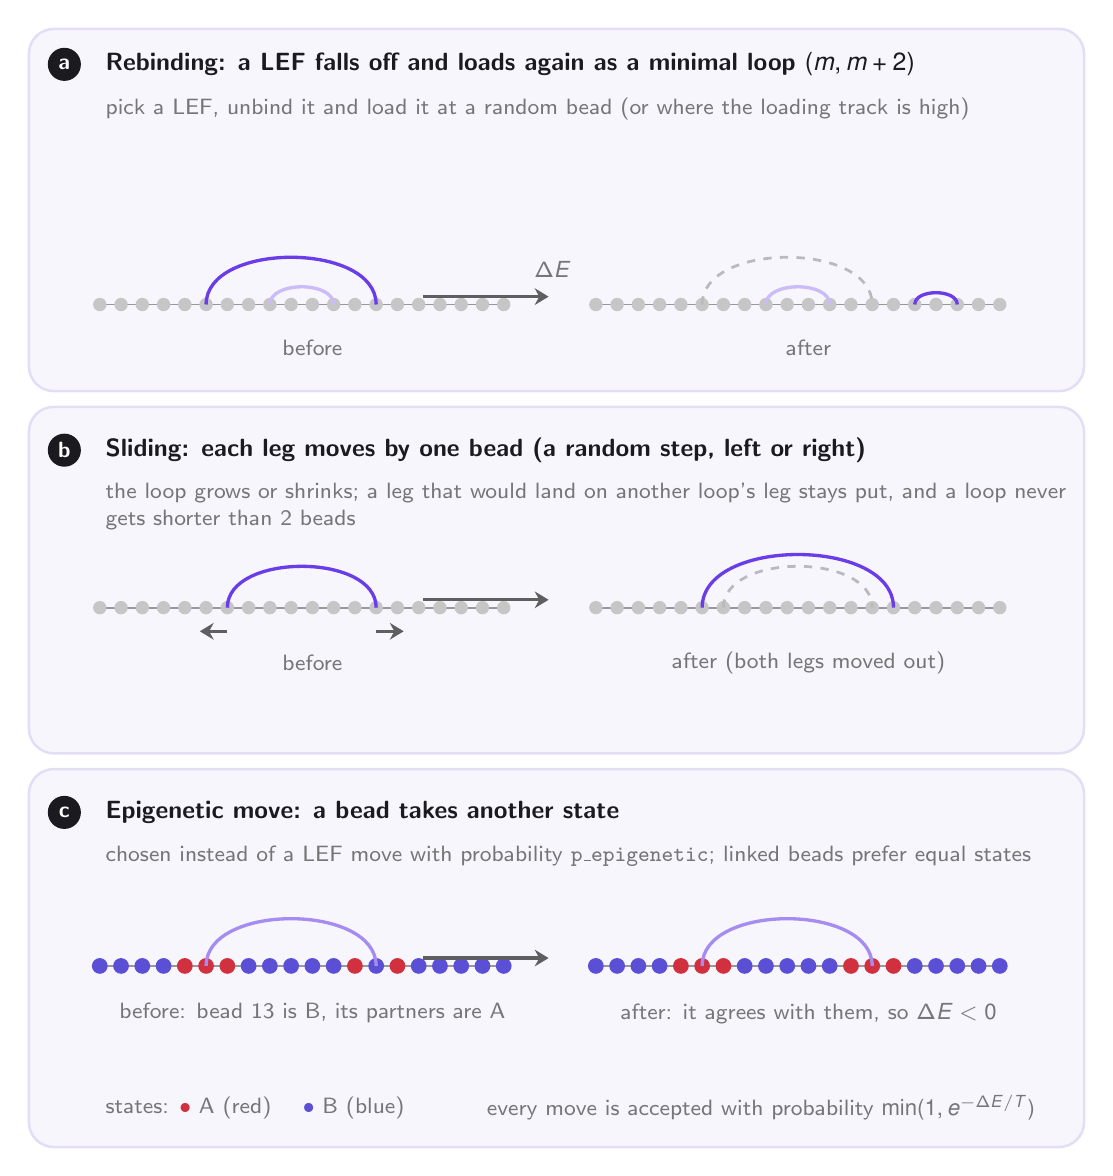
\begin{tikzpicture}
  \panelbg{0}{-0.2}{13.4}{4.4}\panelbg{0}{-4.8}{13.4}{-0.4}\panelbg{0}{-9.8}{13.4}{-5.0}
  \badge{0.45}{3.95}{a}\node[hd] at (0.85,3.95) {Rebinding: a LEF falls off and loads again as a minimal loop $(m, m+2)$};
  \node[note,anchor=north west,text width=12.2cm] at (0.85,3.6500000000000004) {pick a LEF, unbind it and load it at a random bead (or where the loading track is high)};
  \draw[ln] (0.90,0.9)--(6.03,0.9);
  \fill[ink!25] (0.90,0.9) circle (0.085);
  \fill[ink!25] (1.17,0.9) circle (0.085);
  \fill[ink!25] (1.44,0.9) circle (0.085);
  \fill[ink!25] (1.71,0.9) circle (0.085);
  \fill[ink!25] (1.98,0.9) circle (0.085);
  \fill[ink!25] (2.25,0.9) circle (0.085);
  \fill[ink!25] (2.52,0.9) circle (0.085);
  \fill[ink!25] (2.79,0.9) circle (0.085);
  \fill[ink!25] (3.06,0.9) circle (0.085);
  \fill[ink!25] (3.33,0.9) circle (0.085);
  \fill[ink!25] (3.60,0.9) circle (0.085);
  \fill[ink!25] (3.87,0.9) circle (0.085);
  \fill[ink!25] (4.14,0.9) circle (0.085);
  \fill[ink!25] (4.41,0.9) circle (0.085);
  \fill[ink!25] (4.68,0.9) circle (0.085);
  \fill[ink!25] (4.95,0.9) circle (0.085);
  \fill[ink!25] (5.22,0.9) circle (0.085);
  \fill[ink!25] (5.49,0.9) circle (0.085);
  \fill[ink!25] (5.76,0.9) circle (0.085);
  \fill[ink!25] (6.03,0.9) circle (0.085);
  \draw[arc] (2.25,0.9) .. controls (2.25,1.70) and (4.41,1.70) .. (4.41,0.9);
  \draw[arc,cohesin!35] (3.06,0.9) .. controls (3.06,1.20) and (3.87,1.20) .. (3.87,0.9);
  \draw[ln] (7.20,0.9)--(12.33,0.9);
  \fill[ink!25] (7.20,0.9) circle (0.085);
  \fill[ink!25] (7.47,0.9) circle (0.085);
  \fill[ink!25] (7.74,0.9) circle (0.085);
  \fill[ink!25] (8.01,0.9) circle (0.085);
  \fill[ink!25] (8.28,0.9) circle (0.085);
  \fill[ink!25] (8.55,0.9) circle (0.085);
  \fill[ink!25] (8.82,0.9) circle (0.085);
  \fill[ink!25] (9.09,0.9) circle (0.085);
  \fill[ink!25] (9.36,0.9) circle (0.085);
  \fill[ink!25] (9.63,0.9) circle (0.085);
  \fill[ink!25] (9.90,0.9) circle (0.085);
  \fill[ink!25] (10.17,0.9) circle (0.085);
  \fill[ink!25] (10.44,0.9) circle (0.085);
  \fill[ink!25] (10.71,0.9) circle (0.085);
  \fill[ink!25] (10.98,0.9) circle (0.085);
  \fill[ink!25] (11.25,0.9) circle (0.085);
  \fill[ink!25] (11.52,0.9) circle (0.085);
  \fill[ink!25] (11.79,0.9) circle (0.085);
  \fill[ink!25] (12.06,0.9) circle (0.085);
  \fill[ink!25] (12.33,0.9) circle (0.085);
  \draw[ghost] (8.55,0.9) .. controls (8.55,1.70) and (10.71,1.70) .. (10.71,0.9);
  \draw[arc,cohesin!35] (9.36,0.9) .. controls (9.36,1.20) and (10.17,1.20) .. (10.17,0.9);
  \draw[arc] (11.25,0.9) .. controls (11.25,1.10) and (11.79,1.10) .. (11.79,0.9);
  \draw[mv] (5.01,1.0)--(6.60,1.0);
  \node[note] at (6.65,1.35) {$\Delta E$};
  \node[note] at (3.60,0.35) {before};\node[note] at (9.90,0.35) {after};
  \badge{0.45}{-0.95}{b}\node[hd] at (0.85,-0.95) {Sliding: each leg moves by one bead (a random step, left or right)};
  \node[note,anchor=north west,text width=12.2cm] at (0.85,-1.25) {the loop grows or shrinks; a leg that would land on another loop's leg stays put, and a loop never gets shorter than 2 beads};
  \draw[ln] (0.90,-2.95)--(6.03,-2.95);
  \fill[ink!25] (0.90,-2.95) circle (0.085);
  \fill[ink!25] (1.17,-2.95) circle (0.085);
  \fill[ink!25] (1.44,-2.95) circle (0.085);
  \fill[ink!25] (1.71,-2.95) circle (0.085);
  \fill[ink!25] (1.98,-2.95) circle (0.085);
  \fill[ink!25] (2.25,-2.95) circle (0.085);
  \fill[ink!25] (2.52,-2.95) circle (0.085);
  \fill[ink!25] (2.79,-2.95) circle (0.085);
  \fill[ink!25] (3.06,-2.95) circle (0.085);
  \fill[ink!25] (3.33,-2.95) circle (0.085);
  \fill[ink!25] (3.60,-2.95) circle (0.085);
  \fill[ink!25] (3.87,-2.95) circle (0.085);
  \fill[ink!25] (4.14,-2.95) circle (0.085);
  \fill[ink!25] (4.41,-2.95) circle (0.085);
  \fill[ink!25] (4.68,-2.95) circle (0.085);
  \fill[ink!25] (4.95,-2.95) circle (0.085);
  \fill[ink!25] (5.22,-2.95) circle (0.085);
  \fill[ink!25] (5.49,-2.95) circle (0.085);
  \fill[ink!25] (5.76,-2.95) circle (0.085);
  \fill[ink!25] (6.03,-2.95) circle (0.085);
  \draw[arc] (2.52,-2.95) .. controls (2.52,-2.25) and (4.41,-2.25) .. (4.41,-2.95);
  \draw[ln] (7.20,-2.95)--(12.33,-2.95);
  \fill[ink!25] (7.20,-2.95) circle (0.085);
  \fill[ink!25] (7.47,-2.95) circle (0.085);
  \fill[ink!25] (7.74,-2.95) circle (0.085);
  \fill[ink!25] (8.01,-2.95) circle (0.085);
  \fill[ink!25] (8.28,-2.95) circle (0.085);
  \fill[ink!25] (8.55,-2.95) circle (0.085);
  \fill[ink!25] (8.82,-2.95) circle (0.085);
  \fill[ink!25] (9.09,-2.95) circle (0.085);
  \fill[ink!25] (9.36,-2.95) circle (0.085);
  \fill[ink!25] (9.63,-2.95) circle (0.085);
  \fill[ink!25] (9.90,-2.95) circle (0.085);
  \fill[ink!25] (10.17,-2.95) circle (0.085);
  \fill[ink!25] (10.44,-2.95) circle (0.085);
  \fill[ink!25] (10.71,-2.95) circle (0.085);
  \fill[ink!25] (10.98,-2.95) circle (0.085);
  \fill[ink!25] (11.25,-2.95) circle (0.085);
  \fill[ink!25] (11.52,-2.95) circle (0.085);
  \fill[ink!25] (11.79,-2.95) circle (0.085);
  \fill[ink!25] (12.06,-2.95) circle (0.085);
  \fill[ink!25] (12.33,-2.95) circle (0.085);
  \draw[ghost] (8.82,-2.95) .. controls (8.82,-2.25) and (10.71,-2.25) .. (10.71,-2.95);
  \draw[arc] (8.55,-2.95) .. controls (8.55,-2.05) and (10.98,-2.05) .. (10.98,-2.95);
  \draw[mv] (2.52,-3.25)--(2.17,-3.25);
  \draw[mv] (4.41,-3.25)--(4.76,-3.25);
  \draw[mv] (5.01,-2.85)--(6.60,-2.85);
  \node[note] at (3.60,-3.6500000000000004) {before};\node[note] at (9.90,-3.6500000000000004) {after (both legs moved out)};
  \badge{0.45}{-5.55}{c}\node[hd] at (0.85,-5.55) {Epigenetic move: a bead takes another state};
  \node[note,anchor=north west,text width=12.2cm] at (0.85,-5.85) {chosen instead of a LEF move with probability \texttt{p\_epigenetic}; linked beads prefer equal states};
  \draw[ln] (0.90,-7.5)--(6.03,-7.5);
  \fill[B] (0.90,-7.5) circle (0.1);
  \fill[B] (1.17,-7.5) circle (0.1);
  \fill[B] (1.44,-7.5) circle (0.1);
  \fill[B] (1.71,-7.5) circle (0.1);
  \fill[fwd] (1.98,-7.5) circle (0.1);
  \fill[fwd] (2.25,-7.5) circle (0.1);
  \fill[fwd] (2.52,-7.5) circle (0.1);
  \fill[B] (2.79,-7.5) circle (0.1);
  \fill[B] (3.06,-7.5) circle (0.1);
  \fill[B] (3.33,-7.5) circle (0.1);
  \fill[B] (3.60,-7.5) circle (0.1);
  \fill[B] (3.87,-7.5) circle (0.1);
  \fill[fwd] (4.14,-7.5) circle (0.1);
  \fill[B] (4.41,-7.5) circle (0.1);
  \fill[fwd] (4.68,-7.5) circle (0.1);
  \fill[B] (4.95,-7.5) circle (0.1);
  \fill[B] (5.22,-7.5) circle (0.1);
  \fill[B] (5.49,-7.5) circle (0.1);
  \fill[B] (5.76,-7.5) circle (0.1);
  \fill[B] (6.03,-7.5) circle (0.1);
  \draw[arc,cohesin!60] (2.25,-7.5) .. controls (2.25,-6.70) and (4.41,-6.70) .. (4.41,-7.5);
  \draw[ln] (7.20,-7.5)--(12.33,-7.5);
  \fill[B] (7.20,-7.5) circle (0.1);
  \fill[B] (7.47,-7.5) circle (0.1);
  \fill[B] (7.74,-7.5) circle (0.1);
  \fill[B] (8.01,-7.5) circle (0.1);
  \fill[fwd] (8.28,-7.5) circle (0.1);
  \fill[fwd] (8.55,-7.5) circle (0.1);
  \fill[fwd] (8.82,-7.5) circle (0.1);
  \fill[B] (9.09,-7.5) circle (0.1);
  \fill[B] (9.36,-7.5) circle (0.1);
  \fill[B] (9.63,-7.5) circle (0.1);
  \fill[B] (9.90,-7.5) circle (0.1);
  \fill[B] (10.17,-7.5) circle (0.1);
  \fill[fwd] (10.44,-7.5) circle (0.1);
  \fill[fwd] (10.71,-7.5) circle (0.1);
  \fill[fwd] (10.98,-7.5) circle (0.1);
  \fill[B] (11.25,-7.5) circle (0.1);
  \fill[B] (11.52,-7.5) circle (0.1);
  \fill[B] (11.79,-7.5) circle (0.1);
  \fill[B] (12.06,-7.5) circle (0.1);
  \fill[B] (12.33,-7.5) circle (0.1);
  \draw[arc,cohesin!60] (8.55,-7.5) .. controls (8.55,-6.70) and (10.71,-6.70) .. (10.71,-7.5);
  \draw[mv] (5.01,-7.4)--(6.60,-7.4);
  \node[note] at (3.60,-8.1) {before: bead 13 is B, its partners are A};\node[note] at (9.90,-8.1) {after: it agrees with them, so $\Delta E<0$};
  \node[note,anchor=west] at (0.85,-9.3) {states: \textcolor{fwd}{$\bullet$} A (red) \quad \textcolor{B}{$\bullet$} B (blue)};
  \node[note,anchor=east] at (12.9,-9.3) {every move is accepted with probability $\min(1,e^{-\Delta E/T})$};
\end{tikzpicture}
\end{document}
